
\documentclass[11pt, letterpaper]{article}
%\usepackage{bookmark}
\usepackage[a4paper,margin=2cm]{geometry}
\usepackage[]{graphicx}
\usepackage{bm}
\usepackage[strings]{underscore}
\usepackage{apacite}
\setlength{\parindent}{0pt}
\graphicspath{ {./Images} }

\begin{document}
	\begin{titlepage}
		\title{Modelling and Lighting Interior Spaces using Reflected Natural Light}
		\author{Noah Alexiou}
		\date{\today}
		
		\maketitle
		\centering
		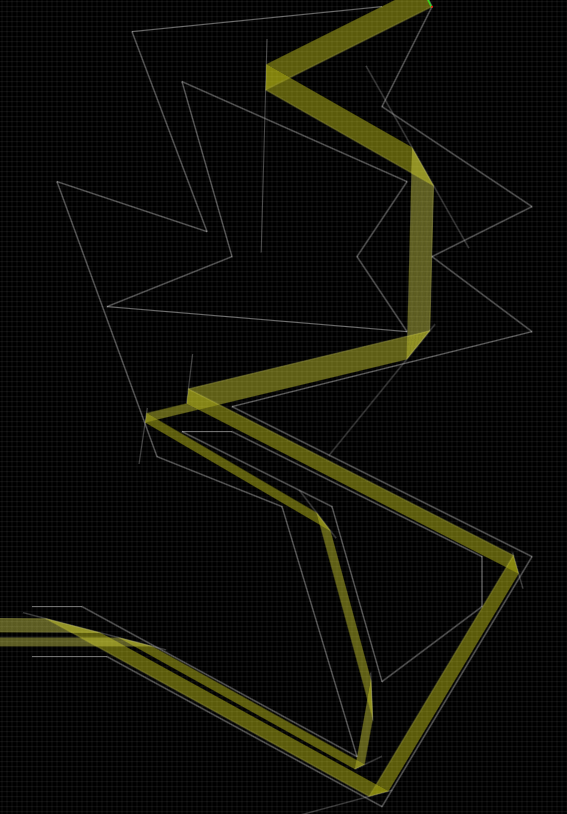
\includegraphics[width=14cm]{cave2.png}
		
	\end{titlepage}
	
	\newpage
	\tableofcontents
	
	
	\newpage
	
	\section{Introduction}
	
	
	\subsection{Premise}
	This study aimed to find optimal mirror placement for minimum decrease in intensity as light travelled throughout a given cave. This was achieved by mapping the cave's geometry and simulating the possible paths of light as a vector throughout the cave with various mirror arrangements.
	
	
	
	
	\subsection{Assumptions} 
	\par
	
	In Order for an accurate solution to be formed, a set of conditions had to be assumed in order to simplify modelling and remove ambiguity.
	\begin{itemize}
		
		\item The given specifications did not provide an orientation, so it was assumed that the cave described was traversed horizontally. This also implied that diagrams depicted the cave 'top-down'.
		
		\item Mirrors and walls of the cave were perfectly parallel to the floor and extended upwards with an undefined height. Light entered the cave parallel to the ground and of equal intensity from floor to ceiling. This simplified modelling and could easily be altered if height was defined. 
		
		
		\item Either light did not decrease in intensity or increase in area according to the inverse square law, or the change was negligible. The suns rays have travelled so far that they can be considered effectively parallel and therefore did not diverge. 
		\cite{yasuda_2024_why}
		
		\item Mirrors reflected light across their entire surface. Light only intersected a mirror and reflected across the normal or did not intersect with a mirror at all.
		
		\item Mirrors were perfectly flat and did not distort or affect light beams in any other way than reflecting them
		
		\item While the entry and exit vectors had no width, it was assumed that light entered the cave through the entire entrance, and could exit throughout the entire exit. Each point along the entrance was considered the beginning of its own vector, with equal direction to the entry vector.  This allowed the entire beams width to be accounted for without introducing unnecessary calculations. 
		
		\item The stimulus implies that the light entering the cave was from the sun, however the sun's position in the sky is constantly changing. Therefore it was assumed that the entry vector's was constant.
		
		
		
	\end{itemize}
	
	\subsection{Observations}
	\par
	
	Insert preamble 
	\begin{itemize}
		
		
		
		
		\item Contaminants in the air may decrease the intensity of light. Distance light travels in cave must be minimised.
		
		\item Mirrors are imperfect and will only reflect a portion of light that hits them.  Therefore the number of mirrors used must also be minimised.
		
		\item Only the edges of each beam of light needed to be found as any light that is within a beam was travelling the same direction as the light at the edges. This allowed intersections with mirrors and cave walls to be found without introducing unnecessary calculations.
		
		\item Light will reflect so that $\textrm{angle  of incidence} = \textrm{angle of refraction}$.
		
		
		\item Clearly paths were not wide enough for a beam of 2 units, the size of the cave's entrance, to pass through them. Therefore the beam was required to be split in order for light to be passed through the cave efficiently.
		
		\item In the case of the beam being split, the edges of each beam were found and each considered the new edge for the split path.
		\newline
		\textbf{ADD DIAGRAM}
	\end{itemize}
	
	
	
	
	
	\subsection{Translation}
	\par 
	
	
		
Light can be modelled as a relative position vector with origin at a mirror surface.
		
Vectors could be modelled on the Cartesian plane and translated without affecting their other properties. 
		
		
		 The scalar product between 2 vectors is a measure of how closely a set of two vectors match each others direction. To find the scalar product, the equation $\textbf{a }\cdot \textbf{b}=|\textbf{a}|\cdot|\textbf{b}| \cdot \textrm{cos}(\theta)$ was used. Clearly for this application, $a$ and $b$ would be listed in traditional component form, When rearranged as $\textrm{cos}^{-1}{(\frac{x_1 \cdot x_2 + y_1 \cdot y_2}{|\textbf{a}|\cdot|\textbf{b}|})} = \theta$ the acute angle between 2 vectors, when arranged tail-to-tail, could be found
		
		 Tools such as desmos mapped vectors as an arrows that span 2 points. This was different than how vectors are usually defined  in component form. The $x$ and $y$ values that usually refer to a direction and magnitude must be converted into 2 discrete sets points, in which one defines the starting point of a vector, and one defines the end. It must be noted that unless explicitly stated, the latter format is what is being used to describe vector position, not regular component form.
		
			As previously mentioned, the intensity of the beam decreased each time light was reflected. The proportion of light remaining after $n$ number of reflections was modelled as the exponential $I=\textrm{Efficiency}^x$, where $I$ is a scalar representation of the intensity of light with respect to the original intensity , $n$ is the number of mirrors, and $\textrm{Efficiency}$ is the percentage efficiency of the mirror in decimal form. Clearly  adding more mirrors will lead to diminishing losses in intensity.
		
		\textbf{INSERT GRAPH}
		
		
	
	
	
	\par 
	
	
	\section{Solve}
	
	\par 
	
		
To map out the cave and its obstacles, the list of conjoined vectors had to be converted into Cartesian co-ordinates. This was achieved through considering the vector sum of the first $n_{th}$ vectors that made up an object from the origin as a new vector, say  $\textbf{a}$. Then taking the sum of $\textbf{a}$ and the $(n+1)_{th}$ vector were added to create a new vector, say $\textbf{b}$. By then taking the Cartesian co-ordinates of the heads of vectors $\textbf{a}$ and $\textbf{b}$ in component form, the head of $\textbf{a} $ can be considered the tail of a new vector, say $\textbf{c}$, and the head of $\textbf{b}$ can be considered the head of $\textbf{c}$. This gives the relative position vector, $\textbf{c}$, of the new wall. These calculations were completed in Excel with vectors in component form. 

\textbf{make a diagram for this one too}
		

		 The co-ordinates of the start and end points of the left wall were arranged into a chain of interconnected $x$, and $y$ co-ordinates and inserted into desmos as lists $X_1$, and $Y_1$ respectively. These lists were than plotted as connected points $(X_1 [J], Y_1 [J])$ where $J$ was an integer ranging from 1, to the length of the given list. The same was repeated for the remaining wall, and obstacle geometry.
		
 
These lists were also manually inserted into the phydemo.app light ray simulator using the text based editor. Values were copied directly from Excel as to not introduce any error.  When the lists were imported as they were, the scale was imperceptibly small, and the $y$-axis was inverted. To solve this, all points had their $x$ components scaled by a factor of 100, and their $y$ components by a factor of -100. Henceforth any mention of points in the context of the phydemo.app simulator will be in reference to these scaled points.

\textbf{tell them what a phydemo is?, mention how the beam works and its normal}


The entry vector and its position were given in component form. After rotating the entry vector by $90^{\circ}$, by swapping its $\textbf{i}$ and $\textbf{j}$ components then multiplying the new j component by -1, and offsetting it so that its tail was positioned at the edge of the cave's right entrance, at $(16, 0)$, plotting it as a relative position vector, by adding its components to the co-ordinates of its tail, the width of its emitted beam perfectly matched that of the width of the entrance. 
		

Once the entry vector was positioned, mirrors were manually placed and adjusted so that they travelled throughout the cave and exited parallel. This began an iterative process with the goal of (in order of priority) reducing light absorbed into the cave walls/resolving collisions, decreasing reflections that the light underwent before exiting, and/or reducing the distance that light had to travel before exiting. 
		

The initial drafted solution required light to undergo 9 reflections in order to reach the exit. This was improved to only 7 in the final revision. The main differences between these solutions was the observation that the path around the first obstacle could be traversed directly without having to divert the beam around the corner, and that a mirror directly before the beam was split was unnecessary and could be removed. These changes not only reduced the number of mirrors required, but also the distance that the beam travelled. No solutions that did not split the beam of light were considered as intentionally losing light was counter intuitive to the task.

\textbf{Insert diagram here}
		
		

Once a satisfactory mirror arrangement was achieved, the start and end points of each mirror were extracted from the phydemo.app simulator and converted back into Cartesian co-ordinates and inserted into desmos as separate lists so the $n_{th}$ element of each list corresponded to the $x$ or $y$ co-ordinate, of either the start or and of the $n_{th}$ mirror. These lists were defined as $x_1$, $y_1$, $x_2$, and $y_2$.

By defining a vector from the $n_{th}$ of each corresponding mirror position list, the mirrors could be depicted in desmos. The same was done but with the 'line' function, rather than the 'vector' function, as to create an object compatible with desmos's intersection and angle measurement tools.
		
 For each entry vector (originating from the left and right sides of the cave's entrance) intersection from the incoming beam of light to the mirror was found and defined as a new vector with components $(x_2 - x_1)\textbf{i}$ and $(y_2 - y_1)\textbf{j}$. This value was then used to find the acute angle between the incoming ray and the mirror $(\theta _1$). The angle between the mirror and the positive $x\textrm{-axis}$ $(\theta _2)$ was also found .
\newline
\textbf{INSERT DIAGRAM}

By performing the operation $- \theta_2 + \theta_1 $, the angle of the new beam could be found. This line was then plotted in polar form with infinite magnitude.
		

In some cases the angle value required multiplication by $-1$ in order for the beam to be travelling in the correct direction.
		

This process was then repeated for all remaining reflections across all paths until of the exiting beam could be found. In order for the exit vector to be $-\textbf{i}$, the angle of the exiting beam must have been $-180^{\circ}$.
		
	
	
	\section{Evaluate and Verify}
	
	\subsection{Reasonableness}
	
 verified that solution was valid through visual inspection in desmos and through checking angle of exit vector
Quantify light gains as exponential
	
	
\subsection{Strengths and Limitations of Solution}
\subsubsection{Strengths}
	
No light was lost through absorption into the cave walls as beam was able to be split. \textbf{state largest opening possible without splitting}

The solution used the minimum amount of mirrors found to be required
	
\subsubsection{Limitations}
	
Beams never come together as they were at the entrance, and exit at incorrect angles. 

Low tolerance for error in mirror placement in case of physical installation, which is imminent considering the context of the task

No investigation into alternative methods of directing light, such as curved mirrors, lenses, or beam expansion/compression.
		
Solution not easily optimisable nor mathematically proven to be the best. The process of synthesising new light paths is not automated nor easily optimisable therefore to iterate on the solution, a significant amount of manual intervention is required
		
		
	
\section{Conclusion}
	
	
\newpage
\bibliographystyle{apacite}
\bibliography{References}
	
\end{document}
